\chapter{評価}
{
\label{chap:eval}
\section{予備評価とその環境}
\label{sec:measure}
\ref{subsec:modeling}節で述べたモデル式を用いて電力を最小化するパイプライン段数とボディバイアス電圧を探索するために予備評価を実施した。表\ref{table:calc_all}は全ての測定に共通する環境である。予備評価で測定した各データについて測定手法と測定結果を示す。

\begin{table}[h]
\centering
\caption{測定環境}
\label{table:calc_all}
\begin{tabular}{|c|c|} \hline
設計 & verilogHDL \\ \hline
プロセス & LEAP65nm/LPT-8 \\ \hline
\multirow{2}{*}{論理合成} & Synopsys Design Compiler \\
& 2016.03-SP4 \\ \hline
\multirow{2}{*}{配置配線} & Synopsys IC Compiler \\
& 2016.03-SP4 \\ \hline
\end{tabular}
\end{table}

\subsection{遅延の見積もり}
\label{subsec:delay_measure}

PE単位で割り当てる演算とボディバイアスを変化させてシミュレーションを行い遅延時間を取得した。シミュレーションした演算の種類は表\ref{table:ALU}に示したものである。さらに、ALUを経由せず、SEのみを経由する場合の遅延時間を取得した。シミュレーション環境を以下に示す。

\begin{table}[h]
\centering
\caption{遅延時間のシミュレーション環境}
\label{table:calc_delay}
\begin{tabular}{|c|c|} \hline
対象 & PE \\ \hline
\multirow{2}{*}{シミュレーション} & Synopsys HSIM \\
& 2012.06-SP2 \\ \hline
電源電圧 & 0.55V \\ \hline
ボディバイアス電圧の範囲 & -2.0V$\sim$ 0.4Vで0.2V毎 \\ \hline
温度 & $25^\circ$C \\ \hline
\end{tabular}
\end{table}

HSIMによるシミュレーションで得られる波形データから遅延時間を求めた。図\ref{fig:delay_wave}に得られたシミュレーション結果の例を示す。ボディバイアスがVBB=-0.6, ADDを演算として割り当てたPEでの波形である。入力方向は南方向、出力方向は北方向であり、入力側の25bitのうち1bit目が変化してから出力側の23bit目が変化するまでの時間を得た。入力側の変化は立ち上がり、立ち下がりの両方を測定し大きい方を最大遅延とした。この例では22.901nsecを最大遅延として取得した。遅延を取得するビット位置の決定方法はSynopsis IC Compilerのタイミング情報を元に決定した。

\begin{figure}[h]
\centering
\includegraphics[width=12cm]{./chap6/fig/delay_wave.eps}
\caption{遅延時間測定のための波形}
\label{fig:delay_wave}
\end{figure}

図\ref{fig:delay_vs_vbb}にADDをマッピングしたPEにおける測定結果を示す。VBBが強いリバースバイアスになるにつれて指数関数に近い変化で遅延時間が増加していることが確認できる。電源電圧を$VDD$、スレッショルド電圧を$V_{th}$とした時$VDD > V_{th}$の領域では遅延時間はボディバイアス電圧に対して多項式的に変化する。一方で$VDD < V_{th}$の領域では遅延時間はボディバイアス電圧に対して指数関数的に変化する。\cite{west}今回のシミュレーションでは$VDD$を0.55Vとしており、$V_{th}$に近い値である。よって、多項式的変化と指数関数的変化の中間的な変化になるため図\ref{fig:delay_vs_vbb}のような変化となる。

\begin{figure}[h]
\centering
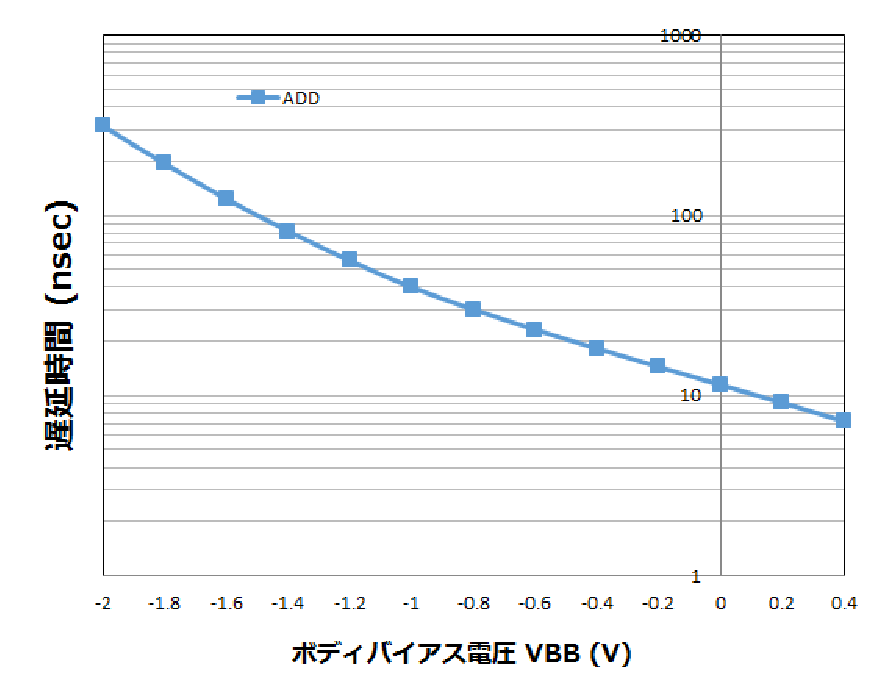
\includegraphics[width=12cm]{./chap6/fig/delay_vs_vbb.eps}
\caption{遅延時間の測定結果}
\label{fig:delay_vs_vbb}
\end{figure}

\subsection{リーク電力の測定}
\label{subsec:leak_measure}

PE\_ARRAYの行単位ー以降ROWと呼ぶーでボディバイアスを変化させてシミュレーションを行いリーク電力を測定した。測定環境を以下に示す。

\begin{table}[h]
\centering
\caption{リーク電力の測定環境}
\label{table:calc_leak}
\begin{tabular}{|c|c|} \hline
対象 & ROW \\ \hline
設計 & verilogHDL \\ \hline
\multirow{2}{*}{シミュレーション} & Synopsys HSIM \\
& 2012.06-SP2 \\ \hline
電源電圧 & 0.55V \\ \hline
ボディバイアス電圧の範囲 & -2.0V$\sim$ 0.4Vで0.2V毎 \\ \hline
温度 & $25^\circ$C \\ \hline
\multirow{2}{*}{入力値} & 全ビットに0 \\ 
& 全ビットに1 \\ \hline
\end{tabular}
\end{table}

\ref{subsec:static_power}節で述べたようにリーク電力はスイッチングしていないにもかかわらず消費される電力であるため、入力値を変化させなかった時に消費される電力をリーク電力とした。ただし、入力値による違いを考慮し全ビットに0を入力した場合と全ビットに1を入力した場合の両方を測定し、その平均値を求めた。測定した結果を図\ref{fig:leak_vs_vbb}に示す。

\begin{figure}[h]
\centering
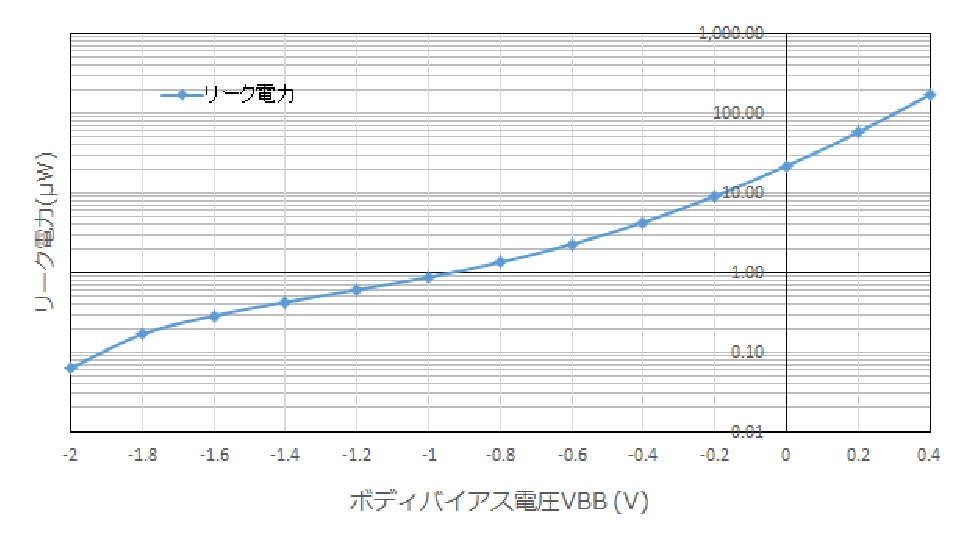
\includegraphics[width=12cm]{./chap6/fig/leak_vs_vbb.eps}
\caption{ROWにおけるリーク電力の測定結果}
\label{fig:leak_vs_vbb}
\end{figure}

\subsection{ダイナミック電力の測定}
\label{dynamic_measure}

アプリケーション実行時のダイナミック電力を測定し、モデル式(\ref{eq:dynamic})で用いるデータを測定した。測定したアプリケーションは表\ref{table:app}に示す4種類である。測定環境を表\ref{table:calc_dynamic}に示す。
\begin{table}[h]
\centering
\caption{シミュレーションしたアプリケーション}
\label{table:app}
\begin{tabular}{|c|c|c|c|} \hline
アプリケーション名 & 内容 & PE使用率(\%) & 使用している行数\\ \hline \hline
af & 24bit(RGB) アルファブレンダ & 75.00\% & 7行\\ \hline
sf & 8bit セピアフィルタ & 83.33\% & 8行 \\ \hline
sepia & 24bit(RGB) セピアフィルタ & 50\%  & 6行\\ \hline
gray & 24bit(RGB) グレースケール & 81.25\% & 8行\\ \hline
\end{tabular}
\end{table}

\begin{table}[h]
\centering
\caption{ダイナミック電力の測定環境}
\label{table:calc_dynamic}
\begin{tabular}{|c|c|} \hline
対象 & PE\_ARRAY \\ \hline
\multirow{2}{*}{電力シミュレーション} & Synopsys Prime Time \\
& 2012.12-SP3 \\ \hline
\multirow{2}{*}{動作シミュレーション}& Cadence NC-Verilog \\
& 10.20-s131 \\ \hline
電源電圧 & 0.55V \\ \hline
パイプライン段数 & 1,2,4,全段 \\ \hline
\end{tabular}
\end{table}

Cadence NC-Verilogを用いてアプリケーション実行時のスイッチング率を求め、Synopsis Prime Timeを用いてダイナミック電力を測定した。測定した結果を表\ref{table:result_dynamic}に示す。

\begin{table}[h]
\centering
\caption{ダイナミック電力の測定結果}
\label{table:result_dynamic}
\begin{tabular}{|c|c|c|c|c|c|} \hline
\multicolumn{2}{|c|}{} & af ($\mu$W/MHz) & sf ($\mu$W/MHz) & sepia ($\mu$W/MHz) & gray ($\mu$W/MHz) \\ \hline \hline
\multirow{4}{*}{$E_{comb}$} & $N_p = 1$ & 50.1430  &  116.5400   & 128.6133  & 46.7077  \\ \cline{2-6} 
							& $N_p = 2$ & 17.8915  & 24.2268   & 30.1860  & 9.6325  \\ \cline{2-6} 
							& $N_p = 4$ & 6.2765  &  8.8185  & 9.2963  & 3.5283  \\ \cline{2-6} 
							& $N_p = 全段$ & 2.68138  & 3.49525  & 2.74738  & 1.44004  \\ \hline
		\multicolumn{2}{|c|}{$E_{clk}$} & 3.73297  & 3.69753  & 3.74962  & 3.76229  \\ \hline
		\multicolumn{2}{|c|}{$E_{reg}$} & 0.26836  & 0.35357  & 0.10738  & 0.08125 \\ \hline
\end{tabular}
\end{table}

\section{評価結果}
\subsection{パイプライン分割の段数と電力最小化の関係}
\label{subsec:stage_vs_power}
4つのパイプライン分割パターン(1段, 2段, 4段, 全段)でボディバイアスを制御し電力を最小化した結果を図\ref{fig:optimization_af}$\sim$\ref{fig:optimization_gray}に示す。

\begin{figure}[h]
\centering
\includegraphics[clip, width=14cm]{./chap6/fig/optimization_af.eps}
\caption{af: 電力最小化の結果}
\label{fig:optimization_af}
\end{figure}


\begin{figure}[h]
\centering
\includegraphics[clip, width=14cm]{./chap6/fig/optimization_sf.eps}
\caption{sf: 電力最小化の結果}
\label{fig:optimization_sf}
\end{figure}


\begin{figure}[h]
\centering
\includegraphics[clip, width=14cm]{./chap6/fig/optimization_sepia.eps}
\caption{sepia: 電力最小化の結果}
\label{fig:optimization_sepia}
\end{figure}



\begin{figure}[h]
\centering
\includegraphics[clip, width=14cm]{./chap6/fig/optimization_gray.eps}
\caption{gray: 電力最小化の結果}
\label{fig:optimization_gray}
\end{figure}

どのアプリケーションにも共通して全段のパイプラインが最も小さい電力となっている。これはパイプライン段数を増やすことによる電力増加が小さい、加えてグリッチの削減とスループット向上のため動作周波数を低くできることによる動的電力の削減効果の方が大きいからである。VPCMAにおいてはパイプライン段数を増やす、つまり各ステージの遅延を小さくすることが有効である。この結果はVPCMAに特有である。他のパイプライン型CGRAにおいてはステージの遅延を小さくするためには使用するPEの数を増やす必要がある。多くのCGRAでは各PEにクロック分配が行われているためステージの遅延を小さくすることによる電力増加はVPCMAに比べて大きい。また、PE内に中間データ保持のためのレジスタを持っていることが多いのでグリッチ削減による電力削減は期待できない。本研究ではパイプライン分割のパターンに制限を設けブルートフォース探索を行った。このことによってアーキテクチャによる違いに左右されずに電力を最小化するパイプライン段数を決定することができるとわかる。しかし、必ずしも全段が電力を最小化するとは限らない。例えばgrayにおいて本研究では考慮しなかった7段で電力が最小になる可能性がある。ゆえに、本手法で粗粒度にパイプライン段数を変化させてブルートフォース探索を行い、その段数の近傍で細粒度に探索を行うことが必要である。


次にアプリケーション間の関係を議論する。grayでは他のアプリケーションと比べて全段にすることによる効果が小さい。この結果からgrayには4段と8段との間にさらに電力を最小化する段数がある可能性を示している。全段にパイプライン分割する有効性と使用するPE\_ARRARYの行数には関係がない。表\ref{table:app}PEの使用率を見るとgrayは使用率、使用行数は大きい。一方で同じ行数を使用するsfでは全段の分割は4段に比べて電力の削減効果は大きい。単純に使用率からではこうした効果は判断ができず本手法はこのようなアプリケーションの依存性に対しても対応できる。

% \begin{table}[h]
% \centering
% \caption{各アプリケーションのPE1つあたりの平均遅延}
% \label{table:average_delay}
% \begin{tabular}{|c|c|c|c|c|} \hline
% & af (nsec) & sf (nsec)  & sepia (nsec) & gray (nsec) \\ \hline \hline
% 遅延時間 & 9.319044667 & 9.938430949 & 12.0477736 & 7.804784017 \\ \hline
% \end{tabular}
% \end{table}


\subsection{ボディバイアス制御の違いによる効果}

次にボディバイアス制御を行うことの効果と行毎の粒度でボディバイアス電圧を制御することの効果について議論する。sepiaにおいてボディバイアス制御を行わずにすべてゼロバイアスとする場合、PE\_ARRAYに一律のボディバイアス電圧を与える場合、行単位でボディバイアス制御をする場合の3パターンでの消費電力を図\ref{fig:comparison_af}に示す。また、各アプリケーション、各段数でのボディバイアス制御をしない場合に対する行単位の制御による平均電力削減率を表\ref{table:reduction_vs_zero_bias}と図\ref{fig:reduction_vs_zero_bias}に、一律制御に対する平均電力削減率を表\ref{table:reduction_vs_uniform}と図\ref{fig:reduction_vs_uniform}に示す。

ボディバイアス制御を行うことで、行わない場合と比べて電力を大きく削減できていることがわかる。図\ref{fig:reduction_vs_zero_bias}からわかるように電力を最小化と明らかになった全段のときに45\%を超える最も高い削減率を示している。段数を増やすと削減率が大きくなっているのは段数を増やせば遅延時間に余裕が生まれリバースバイアスを与えてリーク電力を削減する機会が増えるためである。一方で行単位の制御は一律制御と比べて電力の削減効果が小さくsepia以外1\%に満たない。これは\ref{subsec:stage_vs_power}節で述べたように最小化するときの段数が全段であるからである。本研究でシミュレーションした5MHz$\sim$120MHzの領域では全段の場合、電力を最小化するときのボディバイアスがどの行に対しても-1.6Vなどの強いリバースバイアスを一定に与える場合が多かった。このため、PE\_ARRAYに対して一律のボディバイアス電圧を与える場合と比べて大差がなかった。sepiaが他のアプリケーションと比べて若干削減率が高い理由は行単位の制御にすると使用していない行に強いリバースバイアスを与えることができるからである。6行した使用していないspeiaはこの点で他のアプリケーションと比べ効果が高い。図\ref{fig:reduction_vs_uniform}を見ると電力が最小とはならなかった2段、4段では全段に比べ高い電力削減率となっている。特に2段のときでは18\%を超える削減率を示している。アプリケーションをsf, 段数を2段、要求性能を45MHzとしたときには行単位でボディバイアス制御をすると一律制御と比べて51.14\%の電力削減率が得らた。同様にsfで4段、要求性能110MHzとした場合34.56\%の削減率が得られた。要求性能が高くなると遅延時間を小さくするために0Vに近いリバースバイアスまたはフォワードバイアスを与える必要が出てくる。遅延のボトルネックとなる行は限られているが一律制御の場合は全体に対してフォワードバイアスを与えなくてはならなくなりリーク電力が増大する。一方で行単位の制御ではボトルネックとなる行のみフォワードバイアスを与え、そうではない行には異なるボディバイアス電圧を与えることができる。したがって、要求性能が高い場合には行単位の制御は効果的である。今回は120MHzまでの要求性能しか考慮していないがより高い性能であれば全段でも高い削減率を得られる。ただし、これに関してもアプリケーション依存性がある。なぜならば行単位で遅延のばらつきが発生していないようなマッピングであれば要求性能が高くなっても一律制御で十分だからである。しかし、そういったアプリケーションは稀であるため高い性能が要求される場合は行単位の制御を行うべきである。

\begin{figure}[h]
\centering
\includegraphics[clip, width=12cm]{./chap6/fig/comparison_sepia.eps}
\caption{sepiaにおける電力最小化結果の比較}
\label{fig:comparison_af}
\end{figure}

\begin{table}[h]
\centering
\caption{ゼロバイアス時に対する平均電力削減率}
\label{table:reduction_vs_zero_bias}
\begin{tabular}{|c|c|c|c|c|}\hline
アプリケーション & 1段 & 2段 & 4段 & 全段 \\ \hline \hline
af & 20.88\% &  	37.73\% &  40.60\% &  	46.28\% \\ \hline
sf & 11.25\% &  	35.54\% &  	38.71\% &  	45.34\% \\ \hline
sepia & 14.86\% &  	29.81\% &  	37.01\% &  	46.40\% \\ \hline
gray & 27.02\% &  	44.02\% &  	43.48\% &  	47.15\% \\ \hline
\end{tabular}
\end{table}

\begin{figure}[h]
\centering
\includegraphics[clip, width=14cm]{./chap6/fig/reduction_vs_zero_bias.eps}
\caption{ゼロバイアス時に対する平均電力削減率}
\label{fig:reduction_vs_zero_bias}
\end{figure}

\begin{table}[h]
\centering
\caption{一律ボディバイアス制御に対する平均電力削減率}
\label{table:reduction_vs_uniform}
\begin{tabular}{|c|c|c|c|c|} \hline
アプリケーション & 1段 & 2段 & 4段 & 全段 \\ \hline \hline
af & 11.91\% &  	16.46\% &  	3.25\% &  	0.43\% \\ \hline
sf & 6.77\% &  	18.17\% &  	9.90\% &  	0.80\% \\ \hline
sepia & 8.47\% &  	13.76\% &  	6.82\% &  	1.19\% \\ \hline
gray & 7.14\% &  	13.04\% &  	4.49\% &  	0.76\% \\ \hline
\end{tabular}
\end{table}

\begin{figure}[h]
\centering
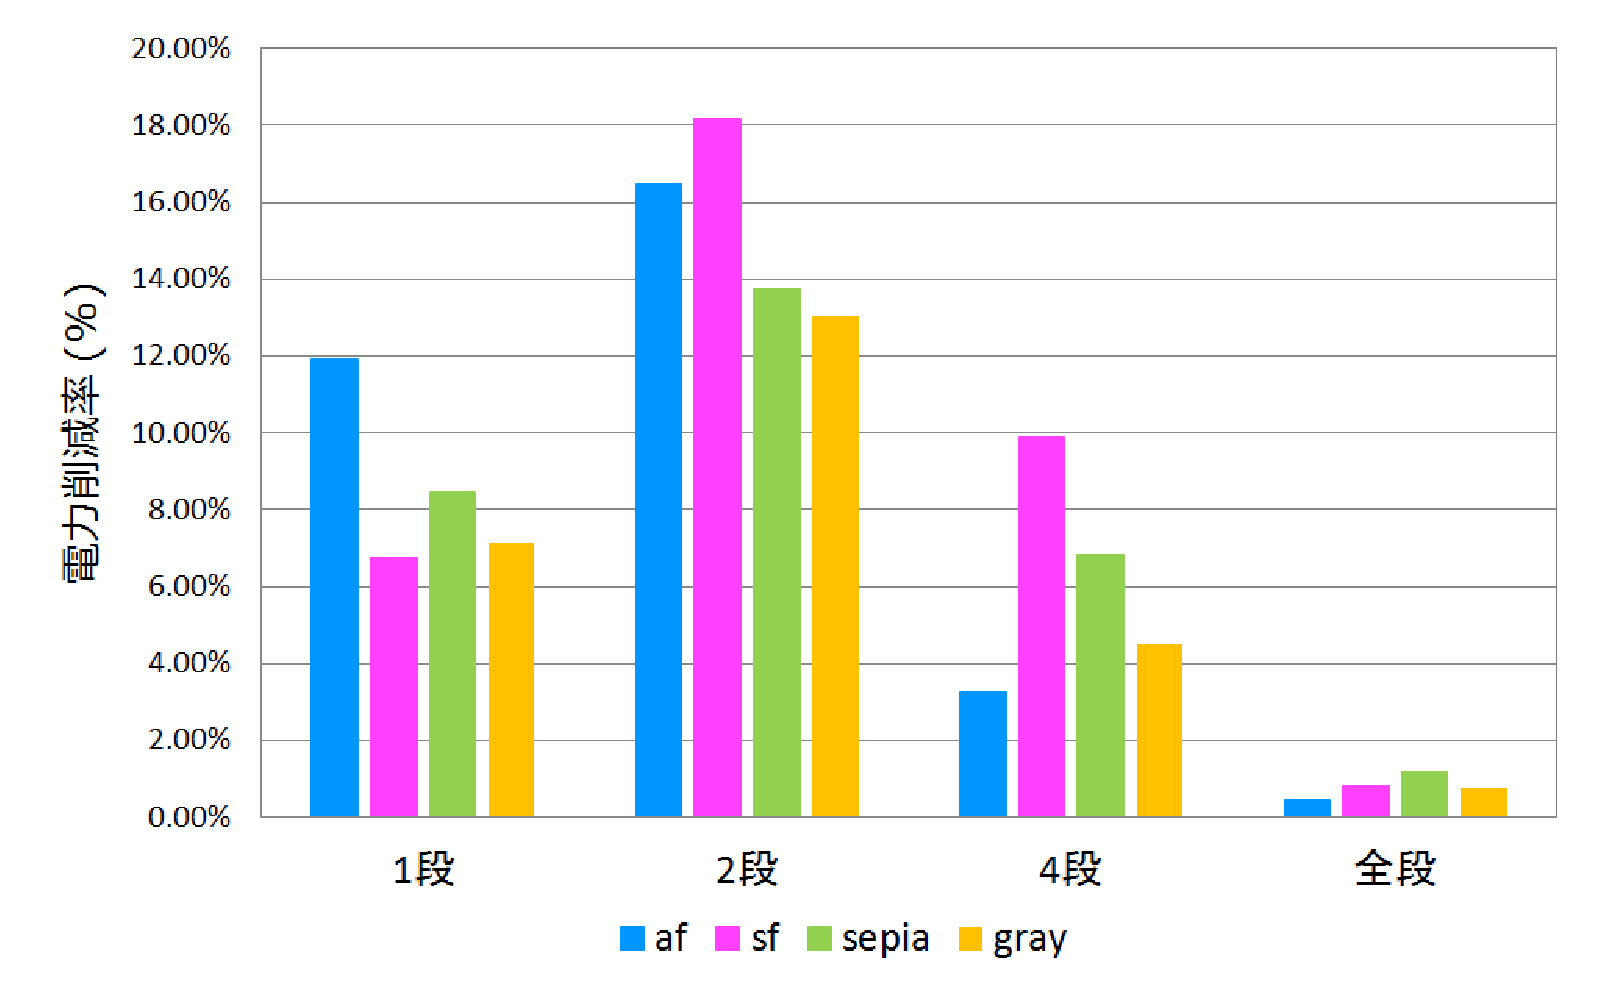
\includegraphics[clip, width=14cm]{./chap6/fig/reduction_vs_uniform.eps}
\caption{一律ボディバイアス制御に対する平均電力削減率}
\label{fig:reduction_vs_uniform}
\end{figure}

}